\documentclass[10pt,twocolumn,letterpaper]{article}

\usepackage{cvpr}
\usepackage{times}
\usepackage{epsfig}
\usepackage{graphicx}
\usepackage{amsmath}
\usepackage{amssymb}

% Include other packages here, before hyperref.

% If you comment hyperref and then uncomment it, you should delete
% egpaper.aux before re-running latex.  (Or just hit 'q' on the first latex
% run, let it finish, and you should be clear).
\usepackage[breaklinks=true,bookmarks=false]{hyperref}

\cvprfinalcopy % *** Uncomment this line for the final submission

\def\cvprPaperID{****} % *** Enter the CVPR Paper ID here
\def\httilde{\mbox{\tt\raisebox{-.5ex}{\symbol{126}}}}

% Pages are numbered in submission mode, and unnumbered in camera-ready
%\ifcvprfinal\pagestyle{empty}\fi
\setcounter{page}{1}

\begin{document}

\title{Human Pose Estimation for Video Game Control}
\author{Rakesh Johny, Tom Li, Aditya Narayanan, Albert Xia}
\maketitle

\begin{abstract}
    Current methods of interacting with computers are flawed in a 
    couple of key ways: they fail to map physically-intuitive motions to their computer 
    control counterparts, and they rely heavily on a user's fine-motor skills, 
    which are heavily impacted by factors such as muscle coordination disabilities 
    and old age. In this paper, we propose a system of computer control through 
    gesture tracking via real-time human pose estimation on an embedded device, 
    which is capable of addresssing these issues, by mapping general physically-intuitive 
    motions into computer control. Furthermore, our device boasts low latency in 
    the human-computer interaction, and is minimally intrustive to the computer being 
    controlled. We test the viability of our system as a computer-control device by playing two 
    video games using only gestures.
\end{abstract}

\section{Introduction}
The human-computer interfaces behind many modern video games use either handheld 
joystick controllers or keyboard and mouse input, which are examples
of typical human input device for computers, monitors, televisions, etc. There are two 
major drawbacks to traditional human input systems that are often overlooked: the input needed 
to achieve a certain effect has little to no correspondence to a physically-intuitive set 
of motions, and more importantly, inputs are heavily dependent on the user's fine motor skills. 
Fine motor skills used to interact with modern technology are heavily affected by factors such 
as muscular coordination disorders and old age. Computer vision, particularly the processes 
of human pose estimation and motion tracking may allow us to create human-computer interfaces 
that link computer control to physically-intuitive human motion inputs with little dependence on 
fine motor ability or additional physical input devices. We propose a vision-based computer-input 
system that maps gestures and motion of the user's body into computer input. We test the system's 
effectiveness with the playability of two simple video games as metrics. In order to demonstrate 
the versatility of our phased-approach to gesture-based control, we select a car-racing game and 
the Google Chrome Dino Racer game as test video games. Such a system, when expanded to replicating 
general keyboard + mouse control, would be instrumental in improving the accessibility of 
modern technology, with implementations far beyond the scope of computer games.

\section{Related Work}
\subsection{Human Pose Estimation}
Some of the largest components of our system fall into the category of so called Human 
Pose Estimation or the ability to properly:

\begin{itemize}
    \item Identify users as sources of input, from a video stream
    \item Segment the user's body to isolate relevant portions of data
    \item Compute the location, in image coordinates, of keypoints on the user's body.
\end{itemize}

The area of Human Pose Estimation is widely studied. There are a wide array of robust, optimized 
solutions for gathering 2D image coordinates of keypoints from images of users. 

\subsubsection{Openpose}
One popular solution to realtime human pose estimation, derived from \cite{8765346}, 
uses Part Affinity Fields (PAFs) to learn to assosciate body parts with individuals in the image, 
and open-source code for the so called openpose library shows promising results for real-time 
human body segmentation. 

\begin{figure}[h]
    \centering
    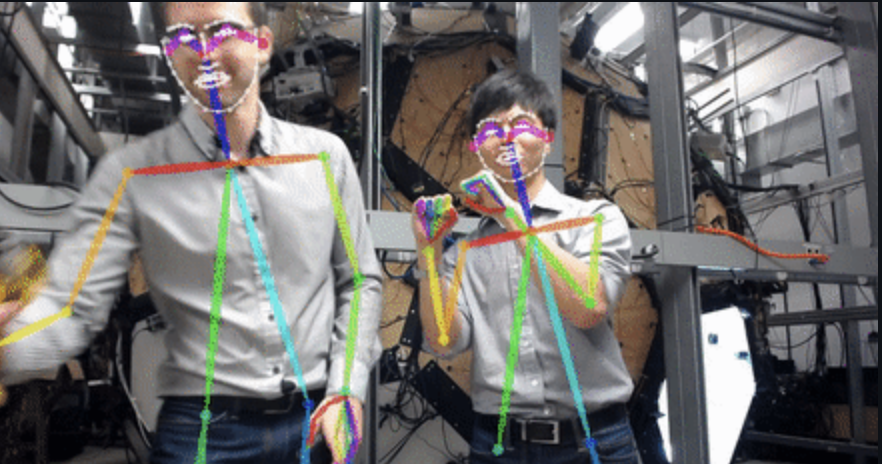
\includegraphics[width = .8\linewidth]{images/openpose.png}
    \caption{A demonstration of openpose performing human body segmentation.}
\end{figure}

\subsubsection{MoveNet and PoseNet}

PoseNet and its more recent counterpart MoveNet are fully convolutional neural network pose 
estimators built on existing ResNet or MobileNet backbones (citation here). Benchmarks of PoseNet and MoveNet show that it is 
viable to run either estimator in real time on embedded devices with appropriate 
model quantizations (citation here), with PoseNet being slightly faster when compared to MoveNet at identical 
levels of quantization. In comparison's with Openpose, PoseNet/MoveNet are shown to perform 
slightly better on instance segmentation of the person class from the COCO dataset.

\subsection{Gesture Identification/Motion Tracking}
Openpose and MoveNet/PoseNet give us promising ways to identify locations of human body features 
(hands, arms, etc.) in a video stream. However, this is not enough to categorize a user's motion 
as a particular command to a computer system. To be able to extract feature motion over time 
as a useful input to our car racing video game, we will have to implement motion tracking 
over a video stream.\\ 

A number of guides exist for implementing feature tracking over video. \cite{tracking_1} 
and \cite{tracking_2} demonstrate simple object tracking across video frames, and \cite{tracking_2} 
demonstrates a system shown to be accurate with motion of hands. We drew on \cite{tracking_1} and 
\cite{tracking_2} in developing a tracking algorithm for the identification of a human user ducking 
or jumping from a keypoint cloud.

\section{Methodology}
Our human computer interface consists of three major steps: Pose Estimation, or feature 
location, Feature Tracking and classification of motions, and video game interfacing. In addition, 
we adopt a multi-phased approach to our human computer interface. Phase 1 consists of a robust and 
general human pose estimator and keypoint detector. The work in Phase 1 is task/game agnostic, as 
we implement identical versions of this phase for the car-racer game as well as the chrome 
dinosaur game. Phase 2 is a game-specific keypoint classifier, where the output from Phase 1 is 
classified into a number of computer commands in a way dependent on the physical motions being 
replicated in the game as well as the computer commands the game is traditionally played with.\\

The motivation behind such a two phase approach rather than building a classifier that directly 
maps input video streams to computer commands is to improve the versatility of our human-computer 
interaction system. A fully general Phase 1 implemented independent of the game in question allows 
the system to be more easily adapted to any particular set of computer commands. We demonstrate the 
versatility of this system through the implementation of our human-computer interface for two 
distinct video games that utilize identical Phase 1 code.

\subsection{Testing Pose Estimation Methods}
Before we develop phase 1 of our human-computer interface, we test a number of proposed solutions 
for human pose estimation to determine which ones are best-suited to our needs. The main criteria 
we require for our human pose estimator are:

\begin{itemize}
    \item Real time operation. The need for this criterion is obvious, as we require low latency 
        classification in order to mimic low-latency commmands for video games. Essentially, the user 
        should feel as if the delay between executing a physical command and the video game reflecting 
        such a command is instantaneous.
    \item The system should be minimally intrusive on the computer used to play the game. This 
        essentially means that we cannot use computing resources so significant that usability of 
        the computer itself is diminished. 
\end{itemize}

\subsubsection{Openpose Python API}
The openpose package offers a Python API for implementing inference over video feeds using one 
of the openpose models. We began testing the openpose Python API for our task, but found that 
installing the API resulted in dependency issues accross multiple team members' computers and 
decided to instead test the openpose pretrained models implemented independently of the openpose 
python API.

%https://learnopencv.com/deep-learning-based-human-pose-estimation-using-opencv-cpp-python/
\subsubsection{Openpose model implemented in OpenCV}
(citation) offers a method to perform inference on CPU/GPU using pretrained versions of the 
openpose hand/body pose estimators. For inference with the openpose pretrained model through 
OpenCV, we observed only 1-2 FPS on a 2.3 GHz Intel i9 CPU. We expect that running the same model 
with CUDA acceleration would result in true real-time performance, but as one of our design 
constraints for our system, we imposed that we cannot use significant GPU resources in order to 
maintain minimal intrusiveness onto the gaming machine.

\subsubsection{PoseNet and the Jetson Nano}
Due to the poor performance of the Openpose models, we began to look at different methods for 
real-time pose estimation. One option that was promising was to completely offload the task of 
human pose estimation to an edge-device to reduce the computational burden on the device used 
to play the games. Such an embedded device would ideally be compact yet powerful enough to run 
quantized versions of pose estimators in real time. We found the NVIDIA Jetson Nano to be an 
ideal candidate for such an embedded device.\\

With a 128-core NVIDIA GPU on a single-board footprint, the Jetson Nano is a popular 
choice for deep model inference on embedded computers. Perhaps more important than the hardware 
itself, however, is the specific Tensor RT optimized models available for use on the Jetson Nano. 
Through a number of optimization techniques such as model quantization, unuzed output elimination 
and horizontal layer fusion/layer aggregation, the Tensorflow with Tensor RT (TF-TRT) backend is 
able to greatly improve inference time on the Jetson Nano. TF-TRT is able to output optimized 
models from Open Neural Network Exchange Format (ONXX) and for popular tasks such as human pose 
estimation, ONXX model formats are readily available from NVIDIA Developers.\\

Using a variant of PoseNet built on a ResNet-18 backbone, we observe 15-17 Frames Per Second 
(FPS) on the Jetson Nano. The so called Pose-ResNet-18-body outputs 17 detected keypoints in 
image coordinate format. 15-17 FPS performance is smooth enough keypoint detection to allow us to 
play games in real time.

\subsection{Pose Estimation}
After testing the variety of available solutions for human pose estimation 
above, we identify that running TRT optimized PoseNet through the Jetson Nano 
is the best solution for our application.\\

To build the first phase of our human-computer interaction device, we use the 
jetson-inference and jetson-utils python packages (citation here) 
to build a human pose estimator in Python. The output of this step is a 
collection of 2D keypoints, correpsonding to image coordinates of the locations 
of the 17 body parts detected by PoseNet.

\subsection{Feature Tracking and Classification}
The second major phase of the human-computer interaction device are the 
keypoint classifiers, which receive 2d image coordinates keypoint detections 
from the pose estimator, and classify collections of keypoints into computer 
commands in a game-specific way. In a fully generalized model of our 
human-computer interaction device, the keypoint "decoder" built in this step 
need not even be a classifier. For more complicated continuous inputs to 
video games, this can be a more complicated regression problem as we would 
seek to estimate continuous output based on the locations of human pose 
keypoints.\\

We construct two distinct keypoint classifiers, one for each video game we 
demonstrate our system on. We construct one classifier to derive a steering 
command from pose keypoints, and one to derive jumping/ducking information 
from an identical set of keypoints.

\subsubsection{Feature Classification For Steering}
The first of two example video games we play as demonstrations of our 
human-computer interface is a simple car-racing game, in which the player's 
vehicle must dodge obstacles by steering left and right. The video game 
accepts controls as either left arrow key or right arrow key, so our 
keypoint classifier for this game seeks to classify collections of keypoints 
derived from our human pose estimator into either steer left or steer right 
commands.\\

To maintain a physical intuition to the gestures that are mapped to either 
left arrow key or right arrow key, we require a user to steer the car with 
an imaginary steering wheel on the video stream. From each frame of the user's 
hands on an imaginary wheel, we extract classifications for the game control 
as follows:

\begin{enumerate}
    \item Assert that both the left wrist and right wrist of the user on the 
        imaginary wheel are present in the frame. If one or more wrists are 
        not present in the frame, skip the remaining steps and output no 
        steering command.
    \item Compute the vector connecting the left wrist of the user to the 
        right wrist of the user.
    \item Compute the angle to the horizontal of the vector computed in step 2.
    \item Threshold on the angle to the horizontal with an experimentally 
        determined cutoff threshold.
\end{enumerate}

Let the location (in image coordinates) of the user's left wrist be $(x,y)$ and 
the location of the user's right wrist be $(x', y')$. The displacement vector 
connecting the two wrists is given by:

$$d = (x - x', y - y')$$

The angle to the horizontal is then given by:

$$\theta = \arctan{\frac{y-y'}{x-x'}}$$

After some experimentation with the system, we found that a reasonable threshold 
for the steering angle is $0.2$ radians. Our classifications for steering angle 
are then derived as:

\begin{itemize}
    \item $\theta > 0.2$: Steer left
    \item $-0.2 < \theta < 0.2$: No command
    \item $-0.2 < \theta$: Steer Right
\end{itemize}

\subsubsection{Feature Classification For Jumping/Ducking} 
The second example video game we demonstrate our human-computer interface system 
on is the Google Chrome Dinosaur Game. The game accepts jumping and ducking commands 
in the form of up arrow key and down arrow key; however, our classifier is a 
little more complex than for the first example video game, as ducking and jumping 
require motion tracking over video to properly classify from human motion. That is, 
you cannot determine from a single frame of video whether or not the user is 
ducking or jumping.\\

In order to deisgn an appropriate classifier for this task, we first establish 
a subset of the keypoints as a more descriptive feature to track. In the case of 
the car steering example, this was done by reducing the set of keypoints to simply 
the left wrist and right wrist. For classification of jumping and ducking, this is 
accomplished by computing a "mean face" or the midpoint of a number of selected 
keypoints. For this application, we select the two eyes, two ears, and the nose, 
and compute the midpoint of these keypoints as our augmented feature to track in 
order to classify whether a user is jumping or ducking. The motivation for establishing 
this feature is to improve the robustness of our classification. Were we to simply 
track a single keypoint such as the nose of the user, our system would not be 
stable against random errors when the nose may not be properly classified or 
may not be classified at all from the phase 1 human pose estimation. Running 
relatively small versions of PoseNet, these types of errors are fairly common. 
Establishing the midpoint of the face as a feature to track allows us to track 
an equally useful but more robust feature.\\

After establishing the midpoint feature, we obtain graphs of the vertical 
position and derivative of vertical position of the midpoint feature over time 
as a user performs jumping and ducking motions in order to develop a game-specific 
classifier for this task. A few methods we considered and our analysis of them 
are given below:

\begin{enumerate}
    \item \textbf{Thresholding on Position}: The most simple method we could 
        employ to classify the movement of the midpoint face into either jumping 
        or ducking would be to threshold on the vertical position in the frame 
        of the midpoint of the users's face. However, this system is not invariant 
        to small motions of the user between jumps and ducks. For example, if the 
        user moves closer to or farther from the camera, this method breaks down.
    \item \textbf{Threshold on Derivative}: One method we considered would be 
        to simply threshold on the derivative of the y-position to discriminate 
        between periods of slow/no motion, and those where the user rapidly moves 
        up or down as one would during a jump or a duck. However, as we can see from 
        the graphs of the derivative over time, both jumps and ducks have periods of 
        high derivative in both the positive and negative direction. i.e) thresholding 
        on the deriviatve is not enough to discriminate between a duck and a jump, although 
        it can discriminate between jump/duck and no command.
    \item \textbf{Template Matching}: From the graph of the derivative over time, we can 
        see that a jump and a duck have inverted profiles on the graph. If we compute 
        the correlation between a template graph for a jump/duck and the current 
        graph at all timesteps, we would be able to discriminate between a jump and 
        a duck effectively. However, this method cannot be used in real time. As we can 
        see from either graph, a jump/duck occupies a significant portion of time. Computing 
        the correlation between a template feature and the motion of the midpoint face 
        in real time would only result in classification at the end of a jump or duck, which 
        would introduct unwanted latency into the system.
    \item \textbf{Threshold on Derivative with extra constraint}: The 
        method we implement in our system is a modification of simply thresholding on 
        the derivative of the y position. We threshold on the vertical position, with 
        the added constraint that at any time $t$, for the sample at that time to be 
        classified as a jump or a duck, the previous $N$ samples of the 
        derivative must be below the threshold. This ensures that only the 
        first period of rapid change in the motion of the midpoint face is 
        captured as a command. $N$ and the threshold are tunable parameters, 
        and in our final system, we set the threshold = $10$ pixels/sec and 
        $N = 3$.
\end{enumerate}

The final solution we implement for our feature tracking/classification for 
the Chrome dino game is as follows:

\begin{enumerate}
    \item For every frame of video, compute $y_t$, the midpoint of all keypoints 
        existing in the frame from the set 
        \{left eye, right eye, left ear, right ear, nose\}.
    \item Compute $y'_t$, the difference of $y_t$ and $y_{t-1}$.
    \item If $y'_t > 10, y'_{t-1} < 10, y'_{t-2} < 10$ and $y'_{t-3} < 10$: 
        Classify current frame as a duck.
    \item If $y'_t < 10, y'_{t-1} < 10, y'_{t-2} < 10$ and $y'_{t-3} < 10$:
        Classify current frame as a jump.
    \item If none of the above conditions are satisfied, classify current frame as 
        no command.
\end{enumerate}

\textit{Note that $y' > 10$ corresponds to a duck and $y' < 10$ corresponds 
to a jump as the image coordinates are zeroed at the top left of the frame.}

\subsection{Game Interface}

\section{Results}

\section{Conclusion and Future Works}

{\small
\bibliographystyle{ieee_fullname}
\bibliography{proposal_bib}
}

\end{document}